\section{测试}

\subsection{正确性测试}
	首先,对于程序的正确性进行测试
	
	\paragraph{expr$\_$to$\_$truthtable\\}
		\lstinputlisting{sources/test_part0.txt}
	\paragraph{truthtable$\_$to$\_$expr\\}
		\lstinputlisting{sources/test_part1.txt}	
	\paragraph{cross$\_$validation\\}
		\lstinputlisting{sources/test_part2.txt}	
\subsection{健壮性测试}
	检测程序对于异常输入的处理	
	\paragraph{expr$\_$to$\_$truthtable\\}
		划分等价类:
		\begin{center}
			\begin{tabular}{cc}
				错误类型 & 抛出异常\\
				空串 & EmptyStringError\\
				非法字符 & InvalidCharError\\
				参数个数错误 & InvalidVariableError\\
				语法错误 & SyntaxError\\
				括号不匹配 & BracketMismatchingError\\
				正常输入 & No Error\\
		\end{tabular}				
		\end{center}

		\lstinputlisting{sources/test_part3.txt}
	\paragraph{truthtable$\_$to$\_$expr\\}
		划分等价类:
		\begin{center}
			\begin{tabular}{cc}
				错误类型 & 抛出异常\\
				空串 & EmptyStringError\\
				非法字符 & InvalidCharError\\
				参数个数$!=2^n$ & InvalidLengthError\\
				正常输入 & No Error\\
		\end{tabular}				
		\end{center}

		\lstinputlisting{sources/test_part4.txt}	
\subsection{效率测试}
	程序运行的速度也是很重要的。
	
	由于8个变量的表达式运行时间过长,我们测试的表达式均采用6个变量。
	
	测试流程如下:
		\begin{itemize}
			\item	随机产生$100$个长度为$2 ^ 6 = 64$的真值表
			\item	对于每个真值表,运用cross$\_$validation的方法,
					将expr$\_$to$\_$truthtable和truthtable$\_$to$\_$expr两个函数都运行一遍
			\item	统计总用时,进而得出长度为$6$时测试数据的平均用时
		\end{itemize}

		\lstinputlisting{sources/test_part5.txt}
	测试结果
	
	选取了20个数据点,根据各部分耗时绘图如下:
	\begin{figure}[h]
		\centering
			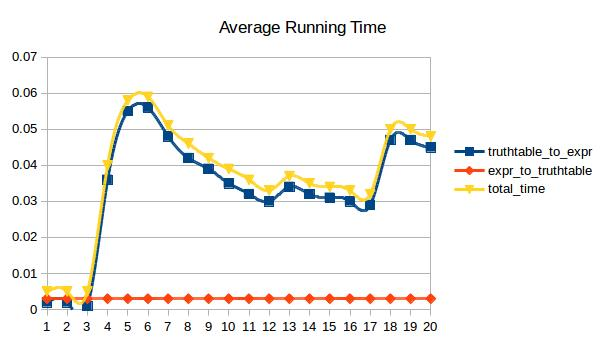
\includegraphics[scale=0.8]{images/speed.jpg}
			\caption{每部分平均耗时(单位:秒)}
	\end{figure}
	
	通过实验表明,程序的主要时间开销在truthtable$\_$to$\_$expr这个函数上。
	
	根据测算,长度为$6$时,平均每条真值表总耗时为$0.048s$,其中truthtable$\_$to$\_$expr耗时$0.045s$,占总耗时的$93.75\%$;
expr$\_$to$\_$truthtable耗时$0.003s$,占总耗时的$6.25\%$
	\begin{figure}[h]
		\centering
			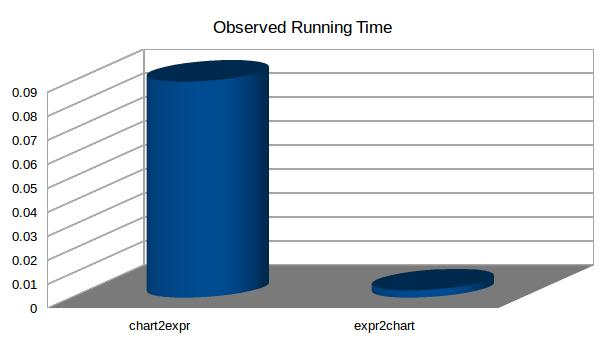
\includegraphics[scale=0.7]{images/result.jpg}
			\caption{两部分平均耗时对比(单位:秒)}
	\end{figure}